\section{Tia Nur Candida (1174086)}
\subsection{Menggunakan LeafletJS dengan MapProxy}
\begin{enumerate}
    \item Run terlebih dahulu Mapproxy
    \hfill\break
    \begin{figure}[H]
		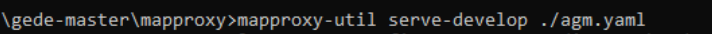
\includegraphics[width=12cm]{figures/Tugas5/1174086/1.png}
		\centering
		\caption{Gambar 1}
	\end{figure}
    \item Buka file basic.html di dalam folder leafletjs di dalam folder gede
    \hfill\break
    \begin{figure}[H]
		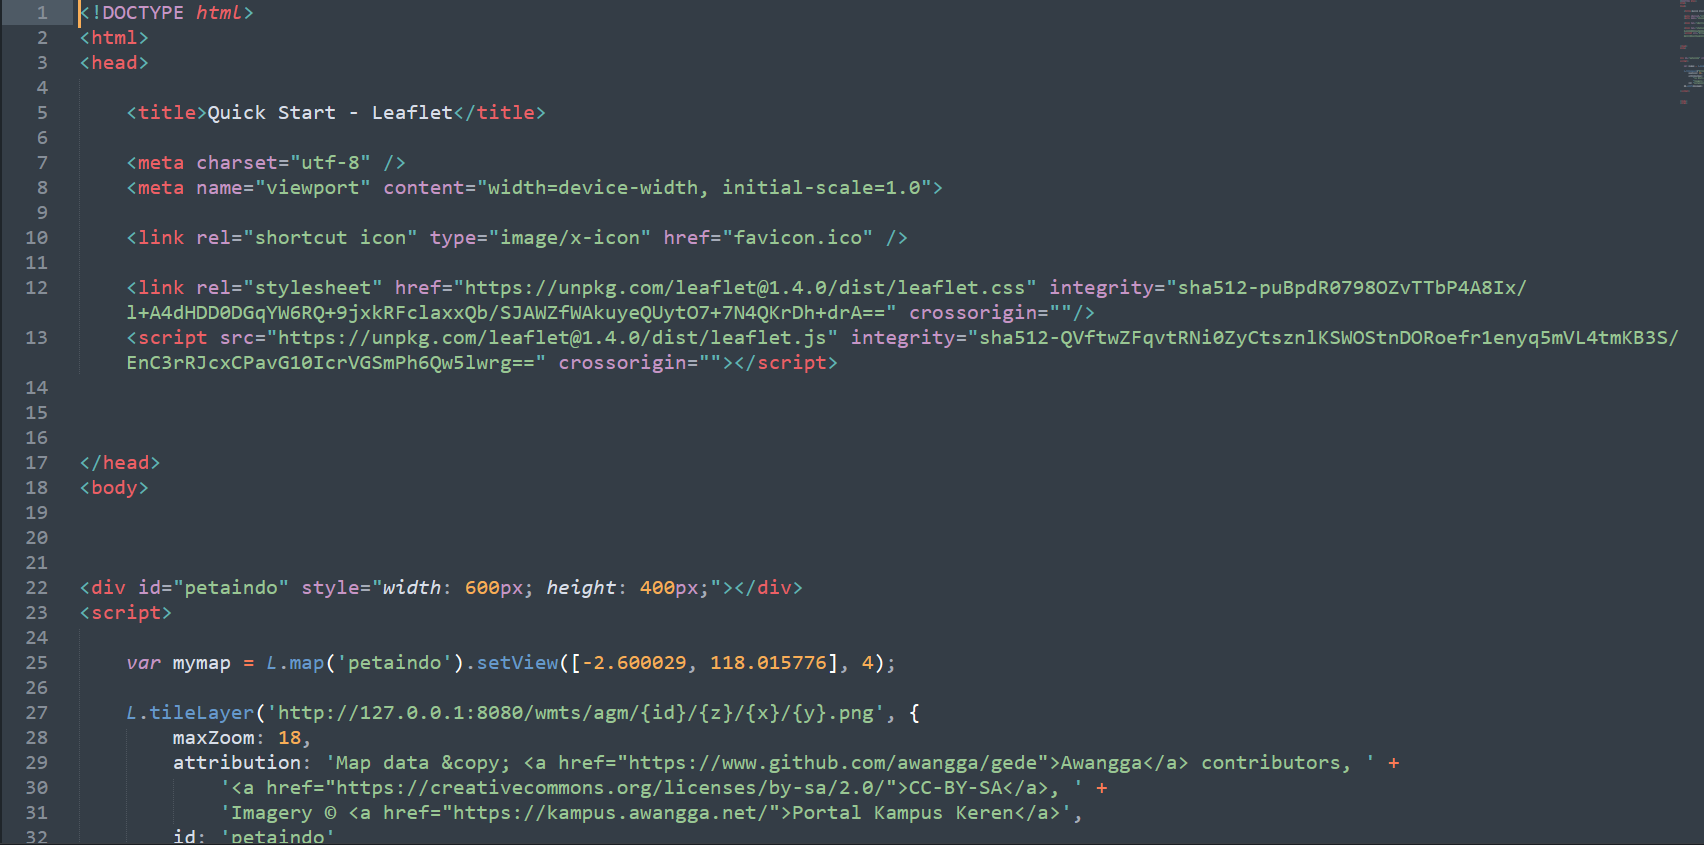
\includegraphics[width=12cm]{figures/Tugas5/1174086/3.png}
		\centering
		\caption{Gambar 2}
	\end{figure}
    \item Lalu buka file tersebut di browser, maka hasilnya akan seperti berikut
    \hfill\break
    \begin{figure}[H]
		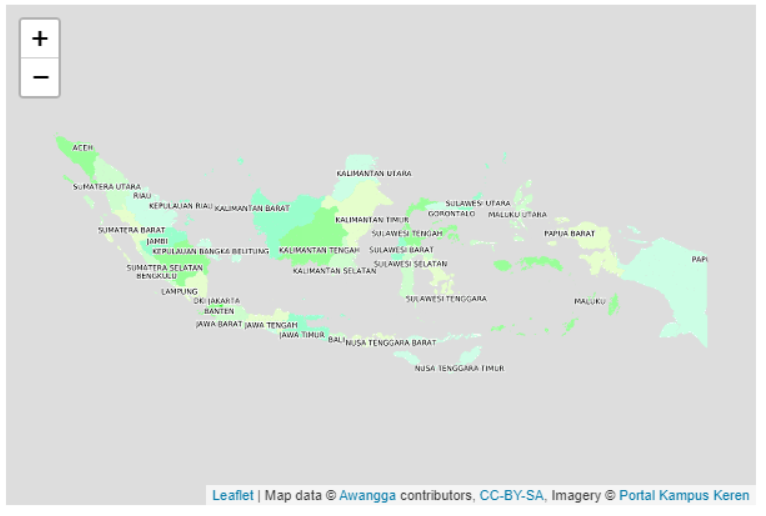
\includegraphics[width=12cm]{figures/Tugas5/1174086/4.png}
		\centering
		\caption{Gambar 3}
	\end{figure}
    \item Pada leafletjs dapat menambahkan marker,circle, ataupun polygon 
    \hfill\break
    \begin{figure}[H]
		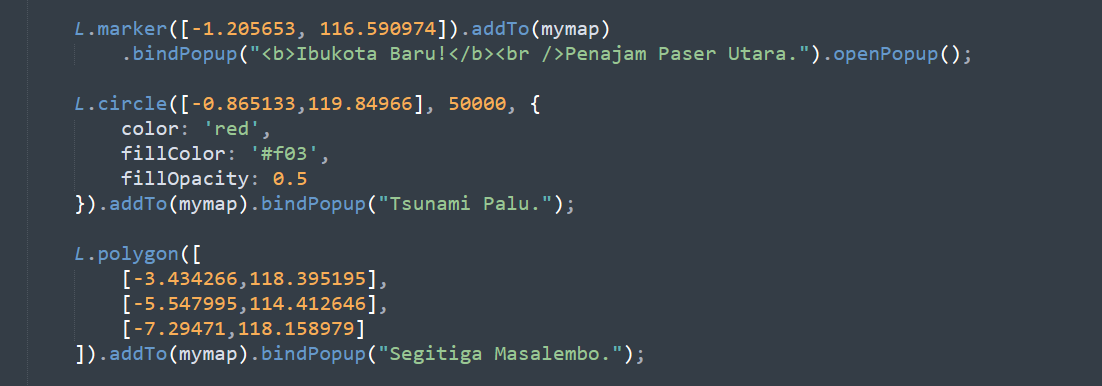
\includegraphics[width=12cm]{figures/Tugas5/1174086/5.png}
		\centering
		\caption{Gambar 4}
	\end{figure}
    \item Lalu buka file tersebut dengan browser dan hasilnya akan seperti berikut
    \hfill\break
    \begin{figure}[H]
		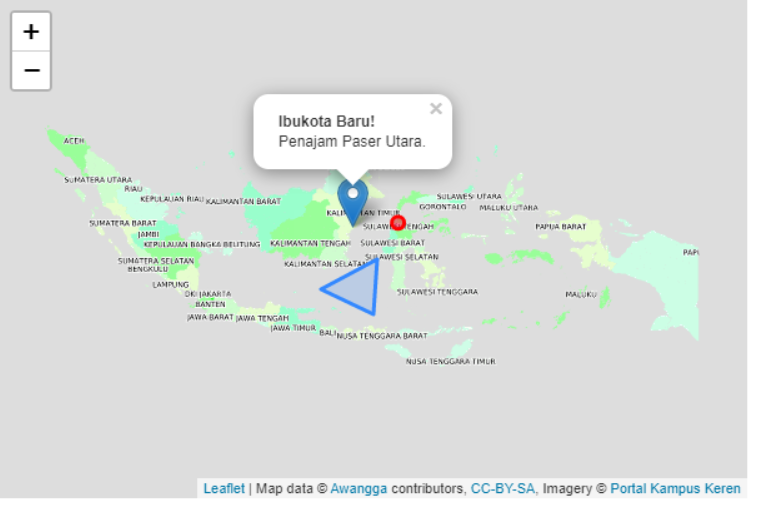
\includegraphics[width=12cm]{figures/Tugas5/1174086/6.png}
		\centering
		\caption{Gambar 5}
	\end{figure}
\end{enumerate}
\subsection{Link Youtube}
https://youtu.be/Qqu4UE9od9w